\section{Overview}

    The Tensor Omics (TOX) tool implements Geometric Learning in a semantic vector space. We represent the data in its natural space, where each measurement is its own axis. We use model-free and minimum-parameter geometric methods to describe the data, find meaningful patterns, identify significant contributions of factors to dependent variables, analyse trajectories, and learn fields of vectors with intrinsic similarity. 

    We rely exclusively on pure linear algebra to characterize these structures, using distances, angles, projections, and linear mapping.

    \vspace{0.5cm}
    Tensor Omics differs from conventional geometric learning tensor decomposition in that it operates in empirically defined semantic vector spaces rather than abstract latent dimensions --- a demonstration (See Figure~\ref{fig:figure1}):

    \vspace{0.5cm}
    (A) Medical omics vectors in semantic space. Each gene, protein or clinical patient measure is placed as a point in multi-dimensional space, with axes representing gene expression in a tissue or clinical patient measures. Arrows denote shift vectors from gene family centroids and enable the explainable detection of changes in gene expression from healthy control. Grid points support interpolation and smoothing. Patient time trajectories are shown in the lower left (healthy controls in green, mean control trajectory in fat light green, and a cancer trajectory in orange). The disease specific signals can directly be obtained by geometric trajectory comparison (violet time resolved shift arrows $\vec{s}_{t_i}$). Significant signals are detected empirically as outliers in the upper 5\%-ile.

    \vspace{0.5cm}
    (B) Angle to the space diagonal as a measure of omics specificity: low angles indicate e.g. broad tissue expression, high angles signal strong tissue preference.

    \vspace{0.5cm}
    (C) Clock hand angle in the Relative Axes Plane (RAP), capturing changes in tissue preference with robust correction for the overall expression magnitude.

    \vspace{0.5cm}
    (D) Causal and explainable omics learning by selecting factors showing geometric similarities in predictive properties. Tensor Omics supports three independent strategies: radial subset growing until only background signal remains (orange), metadata-based selection (e.g. inflammatory response, green), and directional filtering by alignment with a user-defined direction of interest (DOI, e.g. median survival time after treatment or distance of patient trajectory to the healthy control, blue). Methods can be combined to define coherent subfields for geometric analysis.

    \vspace{0.5cm}
    (E) Explainable analysis of patient time trajectories (as shown in A). Changes in tissue preference (angles $\phi$) relative to the anchor axis (AA). Inset plots show the distance to the healthy control trajectory (top) and the angle between consecutive shift vectors (bottom).

    \vspace{0.5cm}
    (F) Learned subfield (see D) characterization by emulating the aggregated effect of vectors on a virtual particle. Measures include signal strength (Frobenius norm $||M||_F$), disease subtyping as directional spread (rank), potential disease specific biomarkers as principal flow direction (first eigenvector of covariance matrix C), and disease specific changes in omics factors as rotation axis and magnitude (from the antisymmetric component ($0.5 \times (C - C^T)$)).

    \vspace{0.5cm}
    (G) Gradient-following kernel traversal to elucidate disease trajectory analysis in early, mid, and late stages: subfield (see D) structure is decomposed via Singular-Value-Decomposition (SVD) into dominant axes (E1, E2 top left) which are smoothed into a single semantic axis (pink line), along which kernel profiles (pink bell top right) reveal flow, rotation, spread, and signal strength (as in F; lower left). Embedding of subfields for machine learning (lower right): The semantic axis is used to orient the subfield with the major flow of the vectors ($\oplus$) and split into five-percentile windows pushed along the semantic axis (dotted lines). Each section is represented by an aggregated vector of field strength (norm), directional spread (rank), principal direction (eigenvector), and rotational moment.

    \vspace{0.5cm}
    (H) The semantic axis (see G) is used to push a higher dimensional object through a lower dimensional space for visualization in the ``Data-Vis'' interactive graphical user interface (Tensor Omics package). This enables direct visualization of higher dimensions and can be used to show for example the developmental hourglass.

    \vspace{0.5cm}
    Panels A–H together illustrate how Tensor Omics unifies geometric learning, empirical explainability, and visualization within a single analytical framework.

    \vspace{0.5cm}
    \begin{figure}[H]\label{fig:figure1}
        \centering
        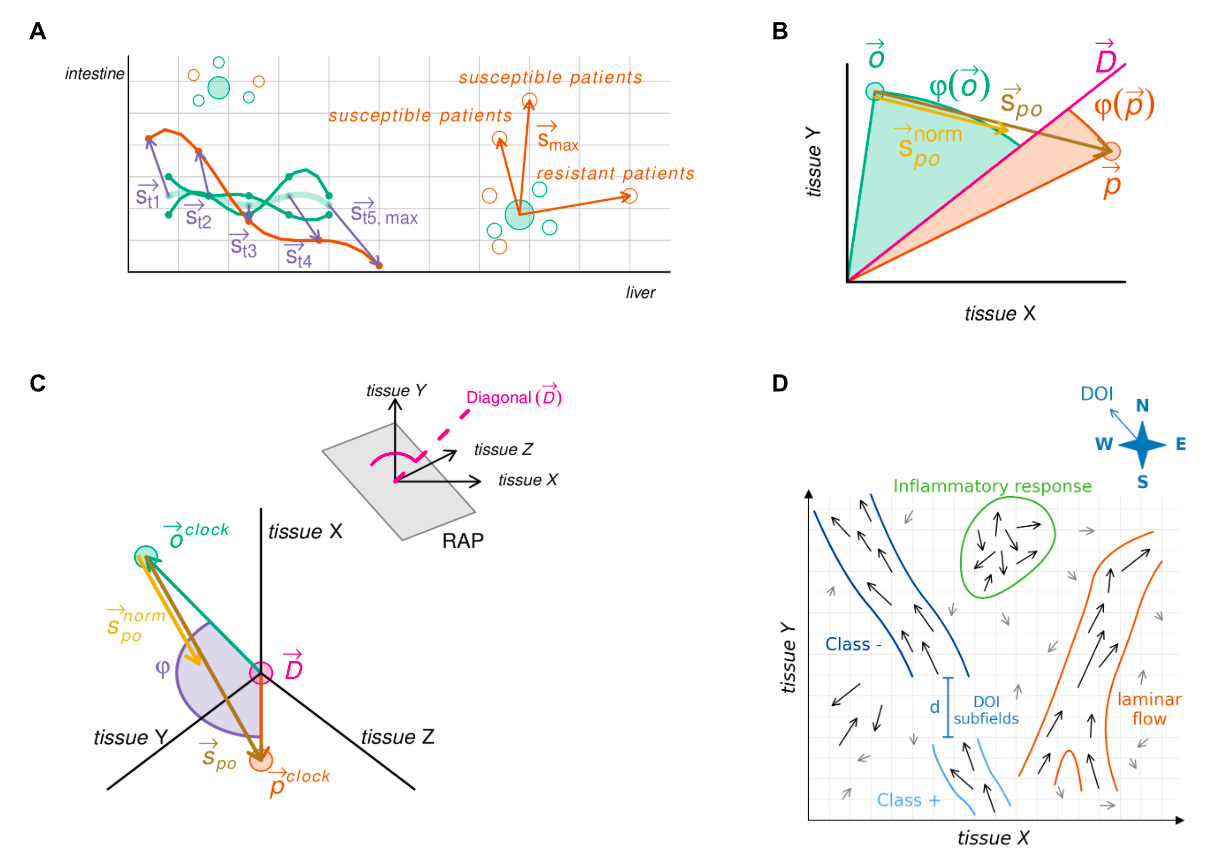
\includegraphics[width=1\textwidth]{figures/tox_methods_1a.png}
    \end{figure}

    \begin{figure}[H]
        \centering
        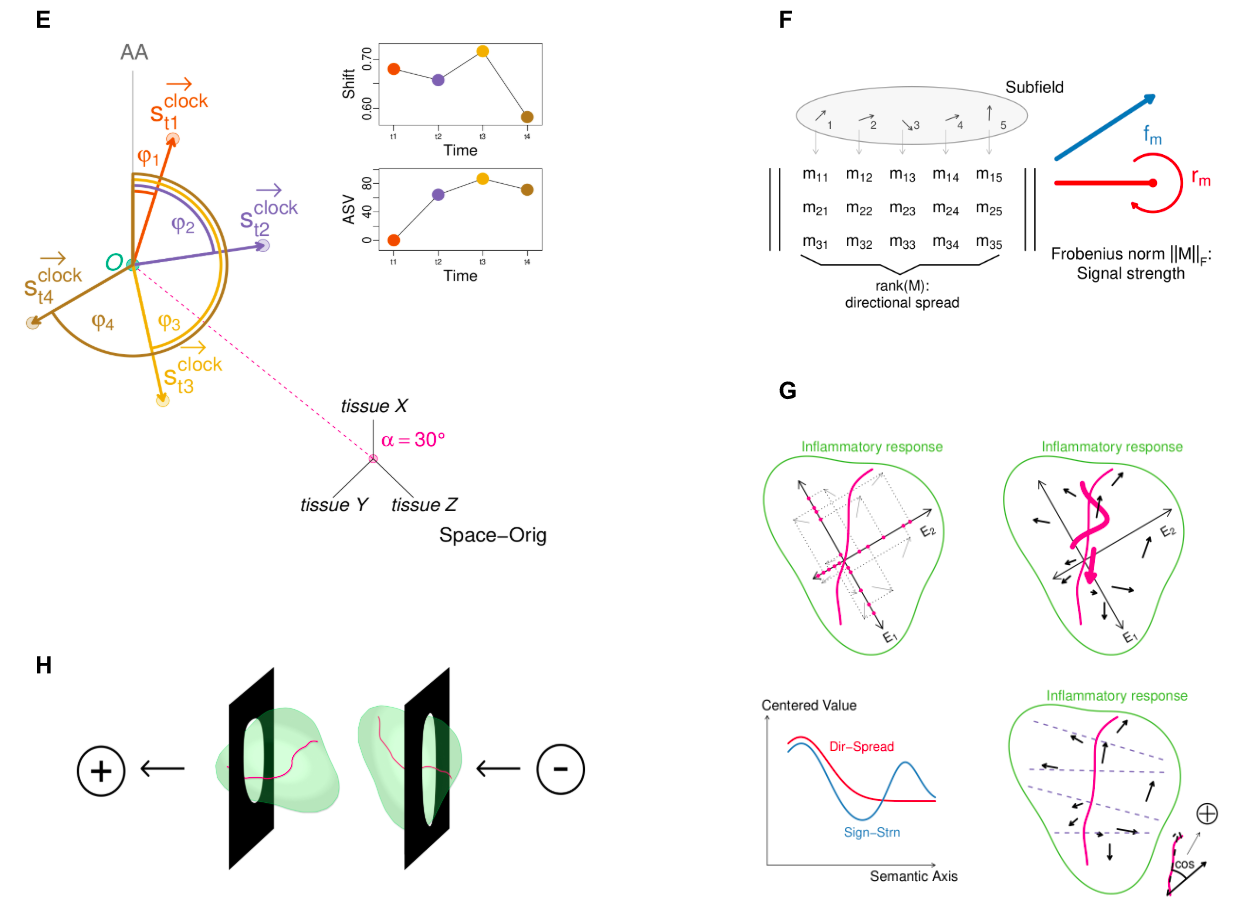
\includegraphics[width=1\textwidth]{figures/tox_methods_1b.png}
        \caption{Overview of the Tensor Omics}
    \end{figure}
